\documentclass{article}

\usepackage{amsmath}
\usepackage{amssymb}
\usepackage{amsthm}
\usepackage{blindtext}
\usepackage{fullpage}
\usepackage{graphicx}

\begin{document}

\begin{figure}
  \centering
  \begin{minipage}[c]{0.45\textwidth}
    \centering
    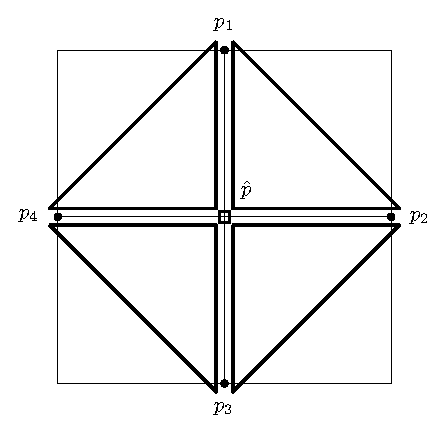
\includegraphics[width=\textwidth]{olim4-stencil.eps}
    \caption{the OLIM4 stencil, consisting of four degree (1, 1)
      triangular updates, and four degree 1 line updates. The
      triangular updates are shown using a slightly exploded diagram
      to ease visualization.}
  \end{minipage}
  \hfill
  \begin{minipage}[c]{0.45\textwidth}
    \centering
    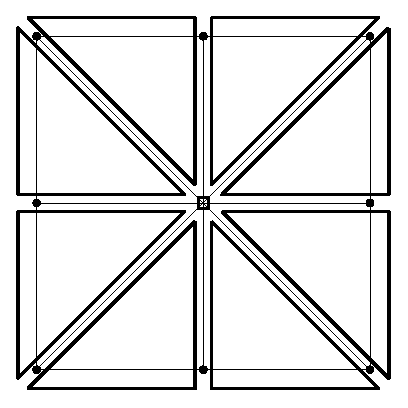
\includegraphics[width=\textwidth]{olim8-stencil.eps}
    \caption{the stencil for the OLIM8 method, which consists of eight
      degree (1, 2) triangle updates, four degree 1 line updates, and
      four degree 2 line updates.}
  \end{minipage}
\end{figure}

\end{document}

%%% Local Variables:
%%% mode: latex
%%% TeX-master: t
%%% End:
